\SubSection{Basic Architecture}

\begin{figure}[t!]
  \centering
  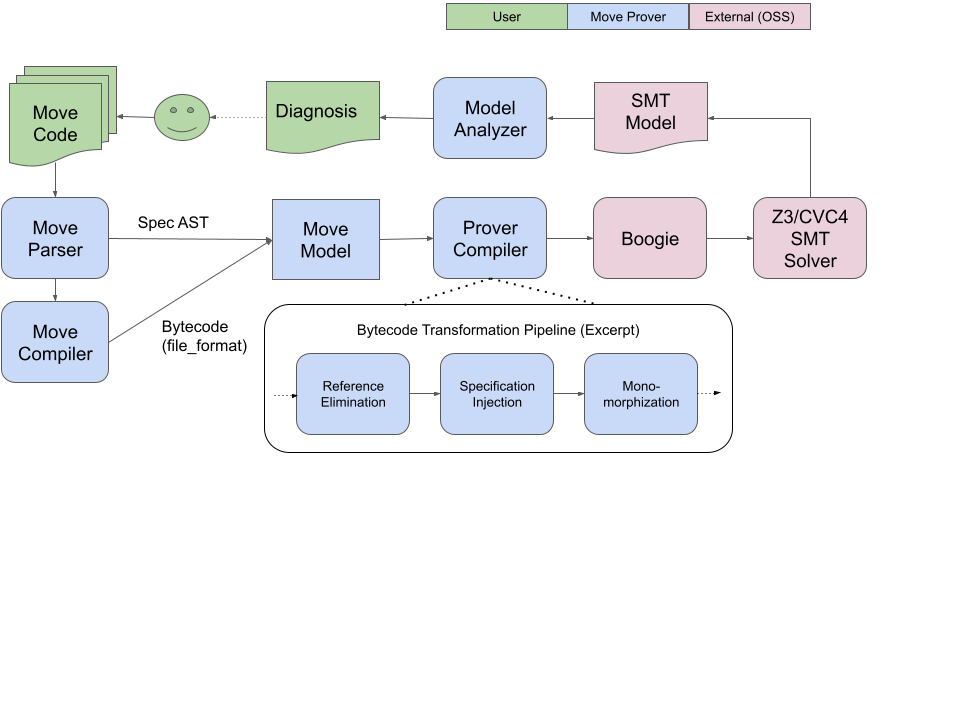
\includegraphics[trim=0 250 0 0, width=\textwidth]{arch.png}
  \caption{Move Prover Architecture}
  \label{fig:Arch}
\end{figure}

The architecture of the Move Prover is illustrated in Fig.~\ref{fig:Arch}. Move
code (consisting of Move programs and specifications) is given as input to the
Move tool chain, which produces two artifacts: the abstract syntax tree (AST) of
the specifications in the code, as well as the translated Move bytecode for the
program part. It is essential that the Prover interprets the Move program on
bytecode level, not on the intermediate AST: this way we verify the ``source of
truth'' which is also executed in the Move VM. Only the specification parts are
passed on as AST. The \emph{Move Model} is a component which merges both
bytecode and specifications, as well as other metdata from the original code,
into a unique object model which is input to the remaining tool chain.

The next phase is the actual \emph{Prover Compiler}, which is implemented as a
pipeline of bytecode transformations. Only an excerpt of the most important
transformations is shown (Reference Elimination, Specification Injection, and
Monomorphization). These transformations will be conceptually described in more
detail in subsequent sections. While they happen in reality on an extended
version of the Move bytecode, we will illustrate them on a higher level of
abstraction, as Move source level transformations.

The transformed bytecode is next compiled into the Boogie intermediate
verification language \cite{BOOGIE}. Boogie supports an imperative programming
model which is well suited for the encoding of the transformed Move code. Boogie
in turn can translate to multiple SMT solver backends, namely Z3 \cite{Z3} and
CVC5 \cite{CVC}; the default choice for the Move prover is currently Z3.

When the SMT solver produces a |sat| or |unknown| result (of the negation of the
verification condition Boogie generates), it produces a model witness. The Move
Prover undertakes some effort to translate this model back into diagnosis which
a user can associate it with the original Move code (as has been illustrated in
Sec.~\ref{sec:RunningProver}.) For example, execution traces leading to the
verification failure are shown, with assignments to variables used in this
trace, extracted from the model. Also the Move Model will be consulted to
retrieve the original source information and display it with the diagnosis.

Subsequently, we will focus on the major bytecode transformations as well as the
encoding and translation to Boogie.


%%% Local Variables:
%%% mode: latex
%%% TeX-master: "main"
%%% End:
